\documentclass[12pt, a4paper]{article}
\usepackage{url,graphicx,tabularx,array,geometry}
\usepackage[utf8]{inputenc}
\usepackage{paralist}
\usepackage{latexsym}
\usepackage{fancyhdr}
\usepackage{ textcomp }
\usepackage{ mathrsfs }
\usepackage{amssymb}
\usepackage{hyperref}

\pagestyle{fancy}

\usepackage{amsmath}
\usepackage{amsfonts}
\usepackage{amssymb}

\DeclareUnicodeCharacter{00A0}{ }

\setlength{\parskip}{1ex} %--skip lines between paragraphs
\setlength{\parindent}{0pt} %--don't indent paragraphs

%-- Commands for header
\newcommand{\bs}{\ensuremath{\backslash}}
\renewcommand{\title}[1]{\textbf{#1}\\}
\renewcommand{\line}{\begin{tabularx}{\textwidth}{X>{\raggedleft}X}\hline\\\end{tabularx}\\[-0.5cm]}
\newcommand{\leftright}[2]{\begin{tabularx}{\textwidth}{X>{\raggedleft}X}#1%
& #2\\\end{tabularx}\\[-0.5cm]}
%\linespread{2} %-- Uncomment for Double Space
\begin{document}
\renewcommand{\headrulewidth}{0pt}
\fancyhf{}
\fancyhead[L]{
\leftright{\textbf{Zusammenfassung}}{Daniel Schmidt}
\line
\leftright{\textbf{Datenbanktheorie SS 16}}{}}
\fancyfoot[C]{\thepage}


\section*{Definition: Datalog Programm}
Ein Datalog-Programm P (ohne IBen(Integritätsbedingungen)) ist eine endliche Menge von Horn-Klauseln mit Jedes $d \in P$ ist entweder
\begin{itemize}
\item ein Fakt $q(...).$ ohne Variable
\item eine sichere Regel $q(...) :- p_1(...),...,p_n(...).$ mit $q\in iPraedikat$
\end{itemize}
Eine Regel heißt sicher, wenn alle in ihr vorkommenden Variablen beschränkt sind.


\section*{Definition: Bedeutung eines Datalog Programms}
Menge der Grundatome, die logisch aus P gefolgert werden können.


\section*{Satz von Gödel / Skolem}
Eine Klauselmenge P hat ein Modell genau dann wenn P hat ein Herbrand-Modell. Daraus folgt, dass ein Verfahren analog zu Wahrheitstabellen in der Aussagenlogik möglich ist.


\section*{Skolemisierung}
Jeder Formel der PL1 Logik, kann in eine erfüllbarkeitsäquivalte Formel in Skolem-Form gebracht werden. Dies bedeutet Pränexnormalform und alle Existenzquantoren durch Funktionen ersetzen.

\section*{Definition: Herbrand-Interpretation}
Eine Teilmenge der Herbrand- Basis

\section*{Grundatom}
Ein Grundatom f ist eine logische Folgerung einer Menge D von Datalog Klauseln (z.B. $D \vDash f$) $\diamondsuit_{Def}$. Jedes Herbrand Modell von D ist auch ein Modell von f.\\
Da f ein Grundatom ist gilt $D \vDash f \Longrightarrow f $ ist in jedem Herbrand-Modell von D enthalten. Das heißt $f \in \bigcap \{ I | I Herbrand-Modell von D \}$.\\
Sei $f \in \bigcap \{ I | I Herbrand-Modell von D \}$, dann ist f ein Grundatom und jedes Modell von D auch in Modell von f. 

\section*{Definition: Mege aller Konsequenzen}
$cons(D) =_{def} \{ f \in HB_D | D \vDash f \}$

\section*{Definition: Substitution}
Eine Substitution ist eine endliche Menge der Form
\begin{equation}
\{ X_1 / t_1, \cdots, X_n / t_n \}, X_1,...,X_n \text{ unterschiedliche Variablen, } t_1,....,t_n Terme, X_i \neq t_i
\end{equation}

Sei $\theta$ eine Substitution, t ein Term (Variable oder Konstante), so gilt \\

\begin{equation}
t\theta =_{def} \begin{cases} t_i, & \mbox{falls } t/t_i \in \theta \\ t, & \mbox{sonst} \end{cases}
\end{equation}

\section*{Definition: Grundsubstitution}
Substitution bei der alle $t_i$ Konstanten sind.

\section*{Definition: Unifizierbar}
Seien $L_1$ und $L_2$ heißen \textbf{unifizierbar}, wenn $(\exists \text{ Substitution } \Theta)(L_1\Theta = L_2\Theta)$. $\Theta$ heißt dann \textbf{Unifikator}.

\section*{Definition: Komposition}
Sei $\Theta = \{ X_1 / t_1, \cdots, X_n / t_n \}, \sigma = \{ Y_1 / n_1, \cdots, Y_m / t_m \}$ Substitutionen. \\
Die Komposition $\Theta\sigma$ von $\Theta$ und $\sigma$ erhält man aus 
\begin{equation}
X_1 / t_1\sigma, \cdots, X_m / t_m\sigma, Y_1 / n_q, \cdots, Y_m / n_m
\end{equation}
Durch Streichen von Elementen der Form Z/Z sowie $Y_i / n_i$ mit $Y_i = X_j$ für ein j$j \in \{1, ..., n\}$

\section*{Definition: allgemeinere Substitution}
Sei $\Theta = \{ X_1 / t_1, \cdots, X_n / t_n \}, \sigma = \{ Y_1 / n_1, \cdots, Y_m / t_m \}$ Substitutionen. \\

Die Komposition $\Theta\sigma$ von $\Theta$ und $\sigma$ erhält man aus $X_1 / t_1\sigma, \cdots, X_m / t_m\sigma, Y_1 / n_q, \cdots, Y_m / n_m$

\section*{Definition: Beweisbaum}
B entsteht aus S durch Anwendung von $\Theta$ auf alle Benennungen von Zielknoten. B repräsentiert einen Beweis für $g\Theta$, g benennung der Wurzel von S.

\section*{Definition: Tiefe eines Baums}
maximale Anzahl von Zielknoten auf einem Pfad von einem Blattknoten zur Wurzel. Entsprechend Knoten der Tiefe i, Ebene i eines Baumes. Zusätzlich: Spezielle Suchbäume (Tiefe 0) für Fakten aus P.

\section*{Suchbaum zu cons}
Sei P ein Datalog-Programm. Die Suchbaum  / Beweisbaum Methode, angewand auf alle Ziele $q(X_1, \cdots, X_{Stelligkeit(q)})$, q intentionales Prädikatesymbol von P, liefert cons(P) als Ergebnis

\section*{Suchbaum, Vollständigkeit}
Die Suchbaum / Beweisbaum Methode bleibt vollständig für ein Programm P, wenn nur Bäume mit max. Tiefe max\_fakt(P) betrachtet werden.

\section*{Resolutionsmethode}
Für allgemeine Klauselformen entwickelte Methode zum automatischen Beweisen.


\section*{Definition: Vollständiger Verband}
Partiell geordnete Mengt $(V, \le)$ bei der zu jeder Teilmenge ein Infinum($\bot_V$) \& Suprenum ($\top_V$)besteht.
Jeder endliche Verband (und jeder Teilmengenverband) ist vollständig.

\section*{Definition: Monotone Transformation}
Abbildung $\tau$ mit $(\forall a,b \in V) (a \le b \Rightarrow \tau(a) \le \tau(b))$.
 
\section*{Definition: Fixpunkt}
$a \in V: \tau(a) = a$

\section*{Magic Set Methode}
Transformiere ein Programm in eine Version, die für ein gegebenes Ziel die gleiche Ausgabe hat aber das Ziel bei bottom-up Auswertung berücksichtigt wird. \href{http://www.is.informatik.uni-kiel.de/~hjk/Datenbanktheorie/Magic_set.pdf}{Algorithmus}, \href{http://www.is.informatik.uni-kiel.de/~hjk/Datenbanktheorie/Magic_Beispiel.pdf}{Beispiel hier.}

\subsection*{Vorgehen}

\subsubsection*{1.Schritt}

Füge für das Ziel $g = q(\cdots)$ die Regel $query^{f\cdots}\footnote{Hochgestellte Zeichen sind Bindungsmuster (wie in Coral)}(X_1, \cdots, X_k) :- q^{\alpha}(\cdots).$ ein, wobei $X_1, \cdots, X_k$ Variablen aus $q^{\alpha}(\cdots)$ sind. Erzeuge für jede Regel $r \in P$ und jedes mögliche Bindungsmuster $\beta$ des Prädikates im Kopf von r eine Regel mit Bindungsmuster für jedes ihrer itensionalen Prädikate. Bestimme dabei unter Beachtung von $\beta$ für jedes Argument im Rumpf ob es ausgezeichnet ist oder nicht. Falls ein IDB-Pr¨adikat im Rumpf mehrfach auftritt, sollte man es durchnummerieren.

\subsubsection*{2.Schritt}

Forme $P^B_g$\footnote{Menge aller erreichbaren Regeln aus Schritt 1} zu $P^{magic}_g$\footnote{Bezüglich g äquivalent}. \\
Sei $P^{magic}_g := P^B_g$. Mach dann für jedes $r \in P^B_g$ und draus folgend für jedes Vorkommen $p^{\beta}\_i(t_1, \dots t_l)$ eines IDB-Prädikates im Rumpf von r folgendes:

\begin{itemize}
\item Streiche alle anderen Vorkommen von IDB-Prädikaten im Rumpf von r
\item Ersetze $p^{\beta}_g$ durch $magic\_r\_p^{\beta}\_i$
\item Streiche alle Variablen aus $(t_1, \dots t_l)$, die nicht ausgezeichnet sind. \footnote{Bei ``Prädikaten'' ohne Argumente die entsthen können: Fall entsprechende Relation $\neq \emptyset$ wahr, sonst falsch}
\item Streiche alle nicht ausgezeichneten EDB-Prädikate aus r.
\item Sei $z^{\alpha}(s_1, \cdots, s_k)$ das Prädikat im Kopf von r. Streiche alle Variablen aus $(s_1, \cdots, s_k)$, die nicht ausgezeichnet sind; $\alpha$ wird nicht verändert. \\
Ersetze $magic\_r\_p^{\beta}\_i(t_1, \dots t_l)$ durch $magic\_z^{\alpha}(s'_1, \cdots s'_{\widetilde{l}})\footnote{Änderungen aus letztem Schritt}$

\item Füge $P^{magic}_g$ die neuen Regeln hinzu
\end{itemize}
\subsubsection*{3. + 4.Schritt}
\newpage
\begin{figure}
\centering
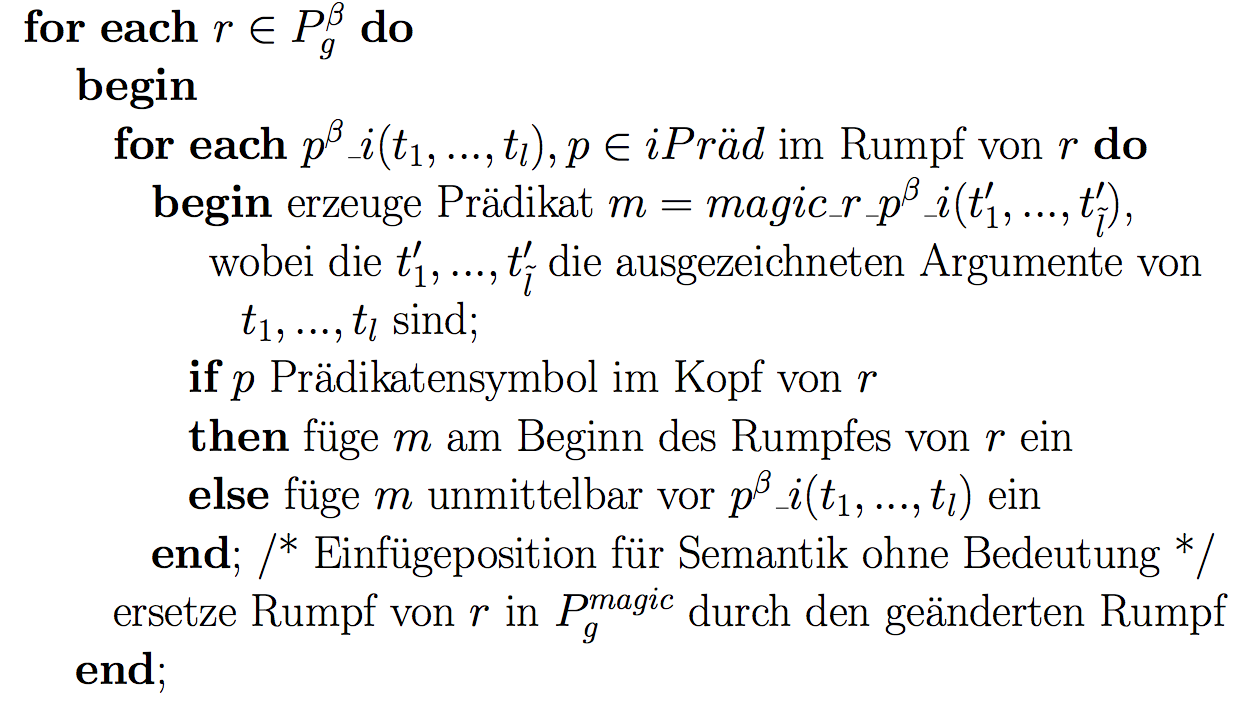
\includegraphics[width=0.95\linewidth]{img/img1}
\caption{}
\label{fig:img1}
\end{figure}

\begin{figure}
\centering
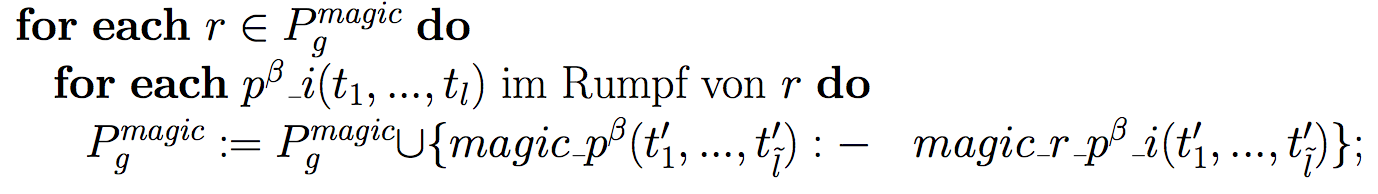
\includegraphics[width=0.95\linewidth]{img/img2}
\caption{}
\label{fig:img2}
\end{figure}

\section*{Definition: Ausgezeichnet}
\subsection*{Argument eines Teilziels}
Konstantensymbol, gemäß $\alpha$ gebunden, es in einem EDB-Prädikat auftritt, das ein ausgezeichnetes Argument hat.

\subsection*{EDB-Prädikat}
Alle seine Argumente sind ausgezeichnet


\end{document}
